\documentclass[dvipdfmx,fleqn]{beamer}
%\documentclass[dvipdfmx,fleqn,handout]{beamer}
\usepackage{amsmath,amssymb,amsthm}

\mode<presentation>
{
  \usetheme{default}
}

\title{\Large Fictitious play}
\author{\large 辻 裕一郎}
\date{\small 2013/6/28}

\usefonttheme{professionalfonts}

\setbeamercovered{transparent=20}

\setbeamertemplate{navigation symbols}{} 
\setbeamertemplate{footline}[frame number] 



\begin{document}

\sffamily
\gtfamily


\begin{frame}
  \titlepage
  \thispagestyle{empty}
\end{frame}

\setcounter{framenumber}{0}


\begin{frame}
\frametitle{はじめに}
\begin{itemize}\setlength{\parskip}{0.5em}
\item
Fictitious playの説明
\item
コードの説明
\item
まとめ
\end{itemize}
\end{frame}


\begin{frame}
\frametitle{Fictitious playの説明}
\begin{itemize}\setlength{\parskip}{0.5em}
\item
2人プレイヤー、戦略が2個の標準形ゲームを考える。

各プレイヤーを0、1とし、戦略も0、1とする。

このゲームを何回も繰り返しプレーするものとする。
\item
各$t$期において、プレイヤー$i(i=0, 1)$は信念$x_{i} (t)$を持っており、「プレイヤー$j(\neq i)$は確率$x_{i} (t)$で戦略1を、$1 - x_{i} (t)$で戦略0をとる」と考えている。

各プレイヤーはこの信念に基づいて期待利得を計算し、期待利得が最大になるように毎期行動するとする。この時の最適反応を$a_{i} (t)$のように表記する。

\end{itemize}
\end{frame}


\begin{frame}
\frametitle{Fictitious playの説明}
\begin{itemize}\setlength{\parskip}{0.5em}
\item
プレイヤーの信念は以下のように形成されるとする。
\[
 x_i(t+1) = \frac{x_i(0)+a_j(0)+a_j(1)+.....+a_j(t)}{t+2}
\]

 このとき、$x_0(t)$ は、
\[
x_0(t+1)
= x_0(t) + \frac{1}{t+2} (a_1(t) - x_0(t))
\]
と再帰的に書くことができる。

これを使い、Pythonで信念の形成のされ方をシュミレーションしてみる。
\end{itemize}
\end{frame}


\begin{frame}[containsverbatim]% verbatim 環境を使えるように
\frametitle{コードの説明}
\begin{itemize}\setlength{\parskip}{0.5em}
\item
Matching pennie gameのコード
\begin{verbatim}
 import matplotlib.pyplot as plt
 from random import uniform

 game_length = 2000 #ゲームの長さを指定
 current_belief0 = uniform(0,1) #最初の信念の指定
 current_belief1 = uniform(0,1)

 def subplots(): #軸、目盛りを設定
    fig, ax = plt.subplots()
    ax.set_yticks([0, 0.25, 0.5, 0.75, 1])
    ax.set_title('Fititious play')
    return (fig, ax)
 fig, ax = subplots() 

\end{verbatim}
\end{itemize}
\end{frame}

\begin{frame}[containsverbatim]
\frametitle{コードの説明}

\begin{verbatim}
 belief0 = [current_belief0] #信念のリストを作成
 belief1 = [current_belief1]

for i in range(game_length):
    if current_belief0 > 0.5: #プレイヤー0の行動を指定
        player0_play = 1
    else:
        player0_play = 0

    if current_belief1 > 0.5: #プレイヤー1の行動を指定
        player1_play = 0
    else:
        player1_play = 1
\end{verbatim}

\end{frame}


\begin{frame}[containsverbatim]
\frametitle{コードの説明}

\begin{verbatim}
#プレイヤーの信念の変更、リストへ追加
    current_belief0 
      = (current_belief0) 
    + ((player1_play - current_belief0)/(i + 2)) 
    current_belief1 
      = (current_belief1)
     + ((player0_play - current_belief1)/(i + 2)) 
    belief0.append(current_belief0) 
    belief1.append(current_belief1)

#信念のリストをプロットする   
 ax.plot(belief0, label = 'x0(t)')
 ax.plot(belief1, label = 'x1(t)')
 ax.legend()
 plt.show()

\end{verbatim}
\end{frame}

\begin{frame}
\frametitle{図1}
\begin{figure}
 \centering
 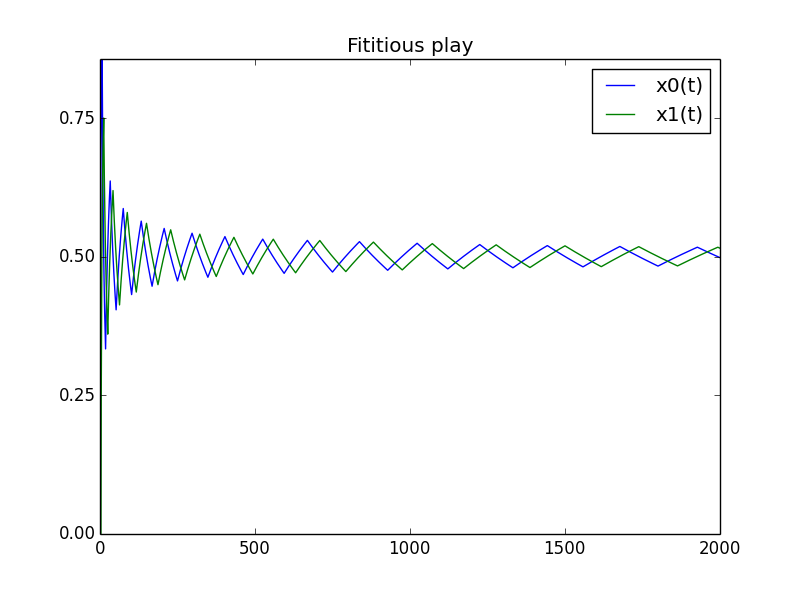
\includegraphics[bb=0 0 240 180, width = 3cm]{fictitious_play.png}
 \caption{Matching pennie game}
 \label{fig:matchingpennies_plot}
\end{figure}
\end{frame}



\begin{frame}
\frametitle{まとめ}
\begin{itemize}\setlength{\parskip}{0.5em}

\item
実際にプログラムを書いて信念の動きをプロットすることで、matching pennie gameではお互いの信念が0.5付近に収束し、coordination gameでは最初の信念$x_{i} (0)$によってお互いの信念が0か1に収束するということがよく分かった。

\item
自分のプログラムの一番の欠点は、汎用性が全くないことである。
利得行列から最適反応が変わる点を計算しなければならない、また戦略が3個以上になっても対応できない。
numpyによる計算にもう少しなれる必要があるな、と痛切に感じた。



\end{itemize}
\end{frame}



\end{document}